\documentclass[journal,10pt,twocolumn]{IEEEtran}
\def\b0{{\bf 0}}
\def\ba{{\bf a}}
\def\bb{{\bf b}}
\def\bc{{\bf c}}
\def\bd{{\bf d}}
\def\be{{\bf e}}
\def\bg{{\bf g}}
\def\bh{{\bf h}}
\def\bi{{\bf i}}
\def\bj{{\bf j}}
\def\bk{{\bf k}}
\def\bl{{\bf l}}
\def\bm{{\bf m}}
\def\bn{{\bf n}}
\def\bo{{\bf o}}
\def\bp{{\bf p}}
\def\bq{{\bf q}}
\def\br{{\bf r}}
\def\bs{{\bf s}}
\def\bt{{\bf t}}
\def\bu{{\bf u}}
\def\bv{{\bf v}}
\def\bw{{\bf w}}
\def\bx{{\bf x}}
\def\by{{\bf y}}
\def\bz{{\bf z}}


\def\bSigma{{\bf \Sigma}}
\def\bA{{\bf A}}
\def\bB{{\bf B}}
\def\bC{{\bf C}}
\def\bD{{\bf D}}
\def\bE{{\bf E}}
\def\bF{{\bf F}}
\def\bG{{\bf G}}
\def\bH{{\bf H}}
\def\bI{{\bf I}}
\def\bJ{{\bf J}}
\def\bK{{\bf K}}
\def\bL{{\bf L}}
\def\bM{{\bf M}}
\def\bN{{\bf N}}
\def\bO{{\bf O}}
\def\bP{{\bf P}}
\def\bQ{{\bf Q}}
\def\bR{{\bf R}}
\def\bS{{\bf S}}
\def\bT{{\bf T}}
\def\bU{{\bf U}}
\def\bV{{\bf V}}
\def\bW{{\bf W}}
\def\bX{{\bf X}}
\def\bY{{\bf Y}}
\def\bZ{{\bf Z}}


%package list
\IEEEoverridecommandlockouts
\let\labelindent\relax
% \usepackage{breqn}
\usepackage{enumitem}
\usepackage{fleqn}
\usepackage{cite}
\usepackage{graphicx}
\usepackage[varg]{newtxmath}
\graphicspath{ {images/} }
\usepackage{pdfpages}
\usepackage{wrapfig}
\usepackage{fancyhdr}
\usepackage{lastpage}
\usepackage{lettrine}
\usepackage{amsmath}
% \usepackage{titlesec}
\usepackage[colorinlistoftodos]{todonotes}
\usepackage{float}
\usepackage[font={footnotesize}]{caption}
\usepackage[numbers,sort,square,compress]{natbib}
\usepackage[para]{footmisc}
\usepackage{xcolor}
\setlength{\belowcaptionskip}{-12pt}
\newcommand{\highlight}[1]{%
  \colorbox{red!50}{$\displaystyle#1$}}

% \usepackage{parskip}
% \setlength{\parskip}{0.02\baselineskip}

% \fancypagestyle{plain}{
%   \fancyhf{} % sets both header and footer to nothing
% \renewcommand{\headrulewidth}{0pt}
%   \fancyhead[C]{2018 International Conference on Indoor Positioning and Indoor Navigation (IPIN), 24-27 September 2018, Nantes, France}% Right header

% }
\pagestyle{plain}% Set page style to plain.

% \pagestyle{fancyplain}
% \fancyhf{}
% \renewcommand{\headrulewidth}{0pt}
% \fancyhead[C]{2018 International Conference on Indoor Positioning and Indoor Navigation (IPIN), 24-27 September 2018, Nantes, France}
\DeclareMathOperator*{\argmin}{argmin}
% \usepackage{titlesec}

% \titlespacing*{\section}{0pt}{1pt plus 2p}{1ex}
% \titleformat*{\section}{\fontsize{12}{12}\bfseries}
% \titleformat{\section}
%        {\normalfont\fontfamily{phv}\fontsize{12}{17}\bfseries}{\thesection}{1em}{}

% \titleformat{\subsection}
%        {\normalfont\fontfamily{phv}\fontsize{12}{17}\bfseries\itshape}{\thesubsection}{1em}{}

\begin{document}
%Here goes the title

\title{Scalar Feedback based Joint Time-Frequency Precoder
  interpolation for  MIMO-OFDM Systems}


%Authors List

 \author{\authorblockN{Author 1, Author 2, Author 3\\}
 \
 \authorblockA{Department of Electrical Engineering\\Indian Institute of Technology Bombay}
% \thanks{Parts of this work was supported by the Bharti Centre for Communication in
% IIT Bombay, and the Visvesvaraya
% PhD Scheme of Ministry of Electronics \& Information Technology,
% Government of India (implemented by the Digital India Corporation).
% }}
}
\maketitle

\thispagestyle{plain}
%Main body starts



% \noindent We consider problem of quantization and interpolation of
% time and frequency varying precoding matrices in wireless MIMO
\begin{abstract}
% In a limited feedback MIMO channel, the performance of the channel can improve significantly if the transmitter knows the channel state information(CSI). The receiver knows the channel information, and it feeds back to the transmitter. However, it is not possible to feedback complete information for a limited-feedback OFDM channel since the channel information for multiple subcarriers consumes a large amount of data. Therefore to resolve this problem, the orthonormality structure of the precoder matrix is exploited to make its one-to-one mapping to a minimal number of scalar parameters. The Precoder matrix is decomposed using Givens Rotation. For an i.i.d. flat-fading Rayleigh channel, these parameters are independent, which makes its quantization and interpolation easy. We propose an efficient method for quantization of the channel state information at the receiver by using adaptive delta modulation for successive time interval. We also propose a method for joint time-frequency interpolation of the channel information at the transmitter. 153-words

  In MIMO-OFDM systems, knowledge of the precoding matrix enables
  effective resource allocation for high rates and low BER. However,
  feeding back precoders for all subcarriers introduces large
  overheads. Past work has shown that the orthonormal structure of the
  precoder enables effective parameterization and quantization using
  Givens rotations and Householder transformations. Also, the use of
  temporal and frequency correlations can further reduce the feedback
  requirements. We present a framework that utilizes adaptive feedback
  with joint time-frequency prediction for precoder construction at
  the transmitter.  Simulations reveal that the proposed method
  achieves significantly lower BERs for various channel profiles
  compared to other approaches.
\end{abstract}

\section{Introduction}
\label{intro}
% no need to write the numbers in your introduction. You start by explaining what is happening currently and then propose your solution.

The use of multiple antennas at the transmitter and receiver can
significantly enhance the performance of wireless systems. Moreover,
in these multiple-input multiple-output (MIMO) wireless systems, the
transmitter can allocate resources more efficiently if the channel
state information (CSI) is made available at the transmitter, both to
improve data rates and to reduce BER~\cite{love2008overview}. To this
end, it is necessary to efficiently feedback the CSI from the receiver 
to the transmitter. In wireless systems that use orthogonal
frequency division multiplexing (OFDM), the feedback needs to be
provided to the transmitter across all subcarriers, and this places a
large feedback demand. However, since the CSI varies gradually in both
time and frequency, effective techniques to reduce feedback overheads
exist, using frequency domain interpolation temporal prediction. In
particular, knowledge of the precoding matrices (that are typically
the orthonormal right singular vectors of the channel matrix) is
essential to achieve link capacity, as well as to parallelize the
channel. In this paper, we focus on the problem of tracking the
precoders of a MIMO-OFDM system across time and frequency for
efficient CSI feedback by tracking a parametrized version of the matrices.

The problem of effective quantization and feedback of precoders for
MIMO-OFDM systems has attracted significant attention in recent
years. Many approaches involve codebook design over the Grassmann
manifold~\cite{mondal2007quantization,schwarz2013adaptive,5946308},
the Stiefel manifold \cite{6891198,Gupt1905:Predictive} and the Flag
manifold~\cite{pitaval2013codebooks}, wherein the manifold structure
of the precoders is used to obtain tangents for predictive
quantization and interpolation across time and frequency. While these
methods have been shown to be very effective for precoder feedback,
they involve operations over higher dimensional manifolds. In
particular, optimization and interpolation is complicated, especially
for manifolds where geodesic paths for interpolation may be difficult
to obtain, especially for joint time-frequency predictive coding. An
alternate approach is to parametrize the precoding matrices using
scalar parameters. The space of unitary matrices parameterized into
independent scalar parameters that correspond to Givens rotations and
Householder transformations of the unitary precoding matrices
\cite{4114278,4556174}. These approaches have been combined with
adaptive delta modulation effectively track precoding matrices both in
the time~\cite{4114278} and frequency domains~\cite{4556174}, albeit
separately.

In this paper, we propose a method for exploiting the joint
time-frequency correlation of the precoder's scalar parameters on the
transmitter using CSI feedback. Typical approaches to predictive
quantization and interpolation do not exploit the joint time-frequency
correlation to enhance the precoder estimate at the
transmitter. However, exploiting the correlations jointly not only
reduces the feedback requirement, but also enhances the precoder
reconstruction accuracy significantly. Further, the independence of
the scalar parameters reduces the problem to one that involves
interpolation of separate scalar valued functions, as opposed to
operations over tangent spaces in
manifolds~\cite{Gupt1905:Predictive}. Simulations reveal that the
proposed method matches the performance of manifold based approaches
with a much lower implementation complexity and fewer number of bits
for quantization.

The rest of this paper is organized as follows: Section~\ref{section2}
describes the system model and the precoder feedback and interpolation
techniques. Section~\ref{section3} compares the BER and achievable
rates for our proposed methods with other approaches. Finally,
Section~\ref{section4} concludes with discussions on future work.

\section{System Model}
For a MIMO-OFDM system with $N_T$ transmitter and $N_R$ receiver
antennas, the channel for the $i$-th subcarrier at time instant $t$
can be modelled as a flat-fading MIMO channel. This flat-fading MIMO
channel can be modelled as
\label{section2}
\begin{equation}
\by_{i,t} = \bH_{i,t}\tilde{\bV}_{i,t} \bx_{i,t}+ \bf{\eta_{i,t}}
\end{equation}
where $\bH_{i,t} \in \mathbb{C}^{N_R \times N_T}$ is the channel
matrix, $\bx_{i,t} \in \mathbb{C}^{N_d}$ is the input data vector,
$\by_{i,t} \in \mathbb{C}^{N_R}$ is the output vector,
$\tilde{\bV}_{i,t} \in \mathbb{C}^{N_T \times N_R}$ is the unitary
precoder, and $\eta$ is the complex additive white Gaussian noise
distributed as ${\mathcal{CN}}(0,I_{N_R})$. We consider the case where
$N_R < N_T$, and the data vector size $N_d = N_R$.  The ``thin'' SVD
(that keeps only those right and left singular vectors that correspond
to non-zero singular values) of $\bH$ is given by
$\bH_{i,t} = \bU_{i,t} \Sigma_{i,t} \bV_{i,t}^{H}$, where
$\bU_{i,t} \in \mathbb{C}^{N_R \times N_R}$,
$\Sigma_{i,t} \in \mathbb{C}^{N_R \times N_R}$ and
$\bV_{i,t} \in \mathbb{C}^{N_T \times N_R}$. $\bU_{i,t}$ and
$\bV_{i,t}$ are matrices whose columns are orthonormal, and
$\Sigma_{i,t}$ contains the singular values
$\sigma_1 \geq \ldots \geq \sigma_{N_R} > 0$ of $\bH_{i,t}$. The
entries of $\bH_{i,t}$ are assumed to be distributed
i.i.d. $\mathcal{CN}(0,1)$. To obtain a precoder at the
transmitter, we need to quantize and feed back information about
$\bV_{i,t}$ for each subcarrier. However, the frequency coherence and
temporal correlations would reduce the overall feedback requirement,
as discussed in subsequent sections.

\subsection{Scalar Parametrization}
\label{givens}
The degrees of freedom in the $\tilde{\bV}_{i,t}$ matrices is smaller
than the number of real entries in the matrix because of the
geometrical structure between the columns of the
matrix~\cite{4114278}. The orthonormal matrix $\tilde{\bV}_{i,t}$ with
$N_T$ rows and $N_R$ columns can be decomposed as
follows~\cite{4114278} (we suppress the $(i, t)$ subscripts in the
decomposition matrices)
\begin{equation}
\tilde{\bV}_{i,t} = \left[\prod_{k=1}^{N_{R}} \bD_{k} \left( \phi_{k,k},\ldots , \phi_{k,N_{R}} \right) \:  \prod_{l=1}^{N_{T}-k} \bG_{N_{T}-l,N_{T} -l+1} \big( \theta_{k,l}\big)  \right] \: \tilde{\bI}
\end{equation}
where $\bD_{k}$ is a diagonal matrix defined as
$\bD_{k}\big(\phi_{k,k}, \ldots, \phi_{k,N_T } \big)$ =
$\mbox{diag}\big( {\bf 1}_{k-1}, e^{j\phi_{k,k}},\ldots,
e^{j\phi_{k,N_T }} \big)$, ${\bf 1}_{k-1}$ represents $k-1$ ones,
and the $N_R \times N_T$ matrix $\tilde{\bI}$ =
$\big[\bI_{N_R }, {\bf 0}_{N_T ,N_T -N_R}\big]^{T}$. Here,
${\bf 0}_{N_T ,N_T -N_R }$ is an $N_T\times (N_T - N_R)$ matrix all of
whose elements are zero. Finally, we also have
\begin{equation}
\bG_{m-1,m}\big(\theta\big)  =
\begin{bmatrix}
\bI_{m-2} & & & \\
& \cos\theta & -\sin\theta & \\
& \sin\theta & \cos\theta & \\
& & & \bI_{t-m}
\end{bmatrix}
\end{equation}
Thus, for a $4 \times 2$ orthogonal matrix $\bV_{i,t}$, we have
\begin{align*}
  \bV_{i,t} & =
  \bD_{1}(\phi_{1,1},\ldots,\phi_{1,4})\bG_{3,4}(\theta_{1,1})
  \bG_{2,3}(\theta_{1,2}) \bG_{1,2}(\theta_{1,3})\times\\
& \bD_{2}(\phi_{2,2},\phi_{2,3},\phi_{2,4}) \bG_{3,4}(\theta_{2,1}) \bG_{2,3}(\theta_{2,2})\tilde{\bI}
\end{align*}
Here, $\phi_{k}$s are referred to as phases, and their collection for
the $i$-th subcarrier at time instant $t$ is captured in a vector
denoted by $\Phi_{i,t}$. $\theta_{l}$s as called rotation angles, and
their collection is captured in a vector referred to as
$\Theta_{i,t}$. We note that $\Phi_{i,t}$ and $\Theta_{i,t}$ represent
the phase and rotation angles for the $i$-th subcarrier at time
instant $t$, as represented in Fig.~\ref{fig:adpm-fig}. It is known
that $\phi_k \in (-\pi, \pi]$ is uniformly distributed between the two
extremes~\cite{4114278}, while $\theta_l$ is distributed
as~\cite{4114278}
\begin{equation}
2l(\sin\theta_l)^{2l-1}\cos\theta_l, \mbox{  }\theta_l \in \left[0, \frac{\pi}{2}\right) \mbox{, } l = 1,2,\ldots,N_T -1
\end{equation}
In addition, $\phi_k$ and $\theta_l$ are statistically independent,
making this representation useful for tracking them separately across
time, as discussed below. The total number of
parameters obtained from the decomposition of a complex orthogonal
matrix $N_{T} \times N_{R} $ is $N_{R}(2N_{T} - N_{R})$. The number of
$\phi_k$ parameters is $N_{R}(2N_{T} - N_{R}-1)/2$ while the number of
$\theta$ parameters is $N_{R}(2N_{T} - N_{R}+1)/2$. Thus, $\Phi_{i,t}$
is a vector of length $N_{R}(2N_{T} - N_{R}-1)/2$, while
$\Theta_{i,t}$ has length $N_{R}(2N_{T} - N_{R}+1)/2$.
\begin{figure}
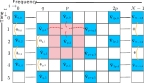
\includegraphics[width=0.5\textwidth]{images/new-adpm.pdf}
\caption{\label{fig:adpm-fig}Subcarriers which need to be
  quantized. In the figure, we see that the subcarrier indicated by
  red arrows has a precoder whose parameters are determined jointly
  using the neighbouring parameters, both in time and frequency.}
\end{figure}

The quantization approach described above is related to the channel
state information feedback present in several wireless standards,
including 802.11ac~\cite{lou2013comparison}, although adaptive
quantization and feedback are not discussed. We show in the further
sections that the use of adaptive approaches can greatly enhance
performance with only very minor modifications to the system.
\subsection{Differential quantization and channel tracking}
\label{quantiz}
For channels that vary slowly with time, adaptive differential
quantization is an effective method for tracking parameters over time
using very few bits (often just one bit per parameter). For example,
while tracking a slowly varying discrete random process $x_n$ at time
$n$, the one bit can be used to determine the direction in which to
move in order to track the parameter. This can be denoted by
$\beta_{n} = \mbox{sign}(x_{n} - \hat{x}_{n-1})$, where $x_n$ is the
unquantized value and $\hat{x}_{n-1}$ is the unquantized (accurate)
value. Further, the step size for the move can be adapted based on the
speed of channel variation as well the accuracy needed. If $\Delta_n$
is the step size, we define our adaptive quantizer as
\begin{equation}
\hat{x}_{n} = \hat{x}_{n-1} + \beta_{n}\Delta_{n} \mbox{ where }
\label{delta_eqn}
\Delta_{n} = \begin{cases}
    M \Delta_{n-1}, & \text{if $\beta_{n} = \beta_{n-1}$}\\
    \Delta_{n-1}/M , & \text{if $\beta_{n} \neq \beta_{n-1}$}.
  \end{cases}
\end{equation}
where $M$ is the increment used during the positive and negative
moves. We initialize $\Delta_1$ as $\Delta_1 = |x_{2}-\hat{x}_1|$. We
note that this is performed separately for each of the quantized
parameters.

To quantize the subcarriers efficiently and exploit the joint
time-frequency interpolation at the transmitter, we select the
subcarriers for quantization in an alternating fashion as shown in
Fig.~\ref{fig:adpm-fig}. The figure shows the channel evolution of an
$N$ subcarrier MIMO-OFDM system with the subcarriers that are
quantized. Every $p$-th subcarrier starting with $0$ is quantized for
even time instances, where, $p$ is the gap between two quantized
subcarrier indices. For odd time instances, subcarriers at the
position $pk+q$ for $k = 0,1,..., \frac{N-1}{p}$ with $q =
{\frac{p}{2}}$.

For the adaptive channel tracking scheme, the arrows in
Fig.~\ref{fig:adpm-fig} show how previous quantized values along with
the 1-bit enhancement are used to find the new quantized value. Since
we use a single bit adaptation, the amount of feedback required is 1
bit for each scalar parameter that is being tracked. On average, this
can be reduced by half if we transmit only $\Theta$ values for
one-time instance and only $\Phi$ values for the next time instant in
an alternating fashion (the untransmitted value is assumed to be the
same as that at the previous instant). In this case, the average
number of bits required to quantize a channel matrix will be
$N_{T}(2N_{T} - N_{R})/2$.

One issue that is associated with the tracking the $\phi_i$ parameters
is that they may change abruptly between $-\pi$ and
$\pi$ due to jumps of $2\pi$. We have avoided this by unwrapping the
phases to facilitate continuous tracking (i.e., we avoid jumps in
phase of magnitude close to $2\pi$).
\subsection{Joint Time Frequency Interpolation}
\label{interp}
After obtaining the $\beta$ values (using the single bit feedback) at
the transmitter, we can construct the precoder at subcarrier indices
$pk$ or $pk+q$, in keeping with the same notation as the previous
section. To construct the rest of the subcarriers, we will use
precoder parameters from both the past and future and time instances
to do the interpolation (using backtracking to ensure causality). In
Fig.~\ref{fig:adpm-fig}, each parameter is interpolated using the
neighbouring subcarriers using bilinear interpolation (equivalent to
linear interpolation in two dimensions). These interpolated values and
then used to reconstruct the precoding matrices all together. Thus,
the approach here is able to exploit the time and frequency
correlation jointly to enhance performance.

One reason why a linear predictive quantization is preferred is
because the underlying parameters can generally be thought to emerge
from an autoregressive (AR) process. For such processes, it is well
known that linear prediction based on past samples is optimal. Even
though the $\Theta$ and $\Phi$ parameters do not manifest as AR
processes, for small changes, a linear approximation works
sufficiently well, as described in~\cite{4114278}, although that
consideration was limited to tracking the temporal evolution of the
parameters.

\section{Simulation and discussion}
\label{section3}
We now present simulations of the scalar feedback based joint
time-frequency predictive quantization outlined in the previous
section. In particular, we analyze the performance of the proposed
quantization and interpolation method for time-varying MIMO-OFDM
systems. The channel is simulated using the typical Jakes Model for
for the COST207 channel power delay
profiles~\cite{molisch2006cost259,cost1989cost}. The BER achieved by
the proposed predictive quantization based precoder is compared
against the ideal precoder for 100 channel evolutions in each run and
averaged. Simulations are performed for normalised Doppler values of
$f_dT_s = 3.41\times 10^{-6}$ (corresponding to a velocity of 37.2 km/h
for $f_c = 1$ GHz) with 1024 subcarriers, and with
$f_dT_s = 1.56 \times 10^{-5}$ (velocity of 172.8 km/h) with 64
subcarriers. The sampling time period $T_s$ was $5\times10^{-8}$
s. For both the situations, we considered $N_T=4$ transmit antennas
and and $N_R=2$ receive antennas. Therefore, the total number of
parameters that determine the precoder is
$N_{R}(2N_{T} - N_{R}) = 12$, with five $\theta_l$s and and seven
$\phi_i$s. We assume that the spacing between fed back subcarrier
indices $p$ to be $33$ and $9$ for the slow and fast channel profiles
respectively (i.e. for the slower channels with 1024 subcarriers, the
subcarriers indices fed back would be $0, 33, 66, \ldots 1023$ and for
the faster channel, with 64 subcarriers, $0, 9, 18, \ldots 63$ would
be fed back).

For the first and the second simulation time instances, since the
precoder is not available at the transmitter, we use 2 bits for
initializing each parameter for effective representation of the
precoder. Therefore, the number of bits for each subcarrier =
$10\times 2$ = 20 (we note that $\phi_0 = \phi_4 = 0$ due to the
non-uniqueness of the SVD). Quantization is performed as given in
Section~\ref{section2}. We note that this is not significant, since,
amortized over long durations, this number becomes small. Subsequent
quantization takes place in the time-domain using one bit for each
parameter. Since the bit budget is small, if the channel varies
sufficiently slowly, either the $\theta_l$ or the $\phi_i$ parameters
are fed back alternately, while retaining the unsent parameters as
being to their previous values, as shown in
Fig.~\ref{fig:adpm-fig}. Here, $\Theta$ is the collection of all
$\theta_l$s and $\Phi$ is the collection of all $\phi_i$s. This brings
down the bit budget to an average of 5 bits(the length of $\Theta$)
and 7 bits (the length of $\Phi$) over alternate feedback instances,
thereby resulting in an average feedback budget of 6 bits.

To enable adaptive tracking of the channel parameters, we start with
an initialization of the step size for each parameter, as discussed in
Equation~\ref{delta_eqn}. The value of $M$ was chosen to be $1.4$, and
can be adjusted appropriately to track the temporal evolution of
parameters for different Doppler frequencies.

Fig.~\ref{fig:error_decay} depicts the rate at which error diminishes
with time for the proposed approach and direct quantization on the
Stiefel manifold using codebooks described
in~\cite{Gupt1905:Predictive}. We see that, since the adaptation of
independent scalar parameters causes the error to decay rapidly, the
error is lower and the convergence is faster, even though the starting
error is higher in the case of the scalar quantization approach. The
independence of the parameters allows the convergence speed to be very
fast. The Stiefel manifold based approach uses nested codebooks that
may be suboptimal when compared to the parametrization using angles.

\begin{figure}
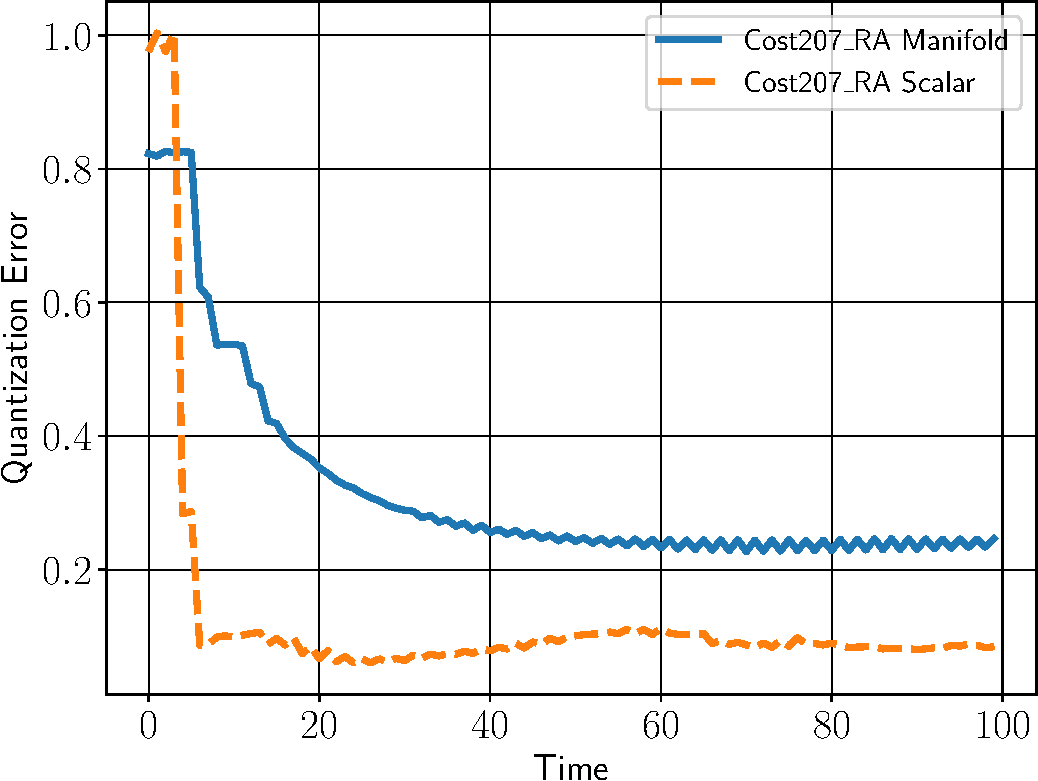
\includegraphics[width=0.5\textwidth]{images/qerror.pdf}
\caption{\label{fig:error_decay}A comparison of the $4\times 2$
  precoder quantization error vs. time instant for the proposed
  approach (labelled ``Cost207\_RA Scalar'') and direct quantization
  on the Stiefel manifold (labelled ``Cost207\_RA Manifold'') for the COST207 channel profile.}
\end{figure}

\begin{figure}
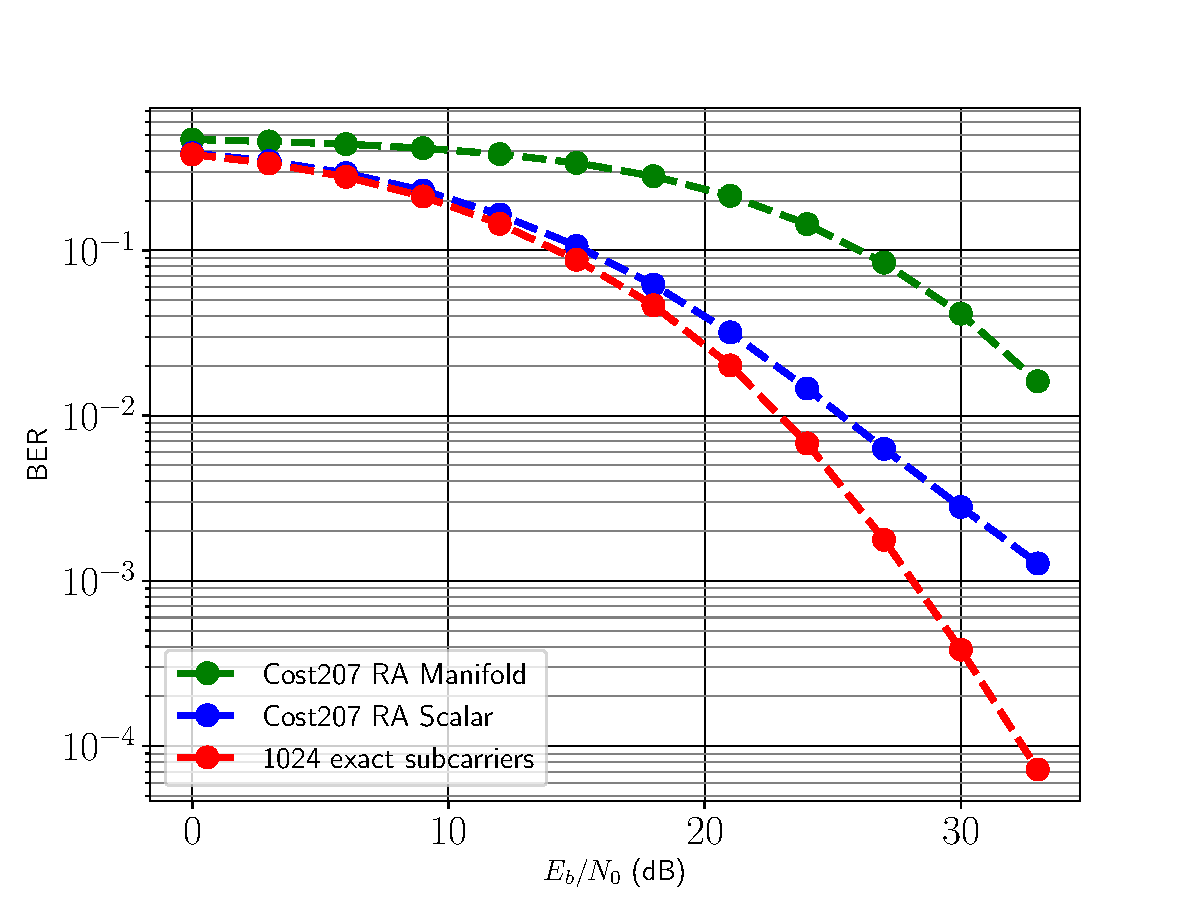
\includegraphics[width=0.5\textwidth]{images/ber1024_035}
\caption{BER vs. SNR for QPSK transmission over the $4\times 2$ 1024
  subcarrier MIMO-OFDM system, with the ITU Cost207-RA channel profile
  for $f_dT_s = 3.41\times 10^{-6}$, corresponding to a velocity of 37.8 km/h.}
\label{fig:ber_ped}
\end{figure}

Fig.~\ref{fig:ber_ped} compares the BER obtained using the proposed
quantization method with that obtained using exact precoders for a
$4\times 2$ 1024 subcarrier system a slow fading
($f_dT_s = 3.41 \times 10^{-6}$). We can observe that the performance
of the proposed method tracks the performance with exact precoders for
a wide range of SNRs. This can be attributed to the fact that even the
1-bit update to the scalar parameters is able to approximate the
precoder very accurately. Since the channel variation across
subcarriers is gradual, owing to the limited delay spread of the
channel profile, linear interpolation and prediction yields good
performance. Moreover, this method outperforms the Stiefel manifold
based approach due to the fact that the adaptation is much more
accurate for scalar parameters than the tangent space based adaptation
used over the Stiefel manifold, and the outperformance is in excess of
10 dB. The gap from the optimal precoder performance narrows further
when the speed reduces.

Fig.~\ref{fig:ber_veh} shows a similar comparison for a similar
situation with a higher speed. The faster variation of the channel
taps with time necessitates the use of a smaller number of subcarriers
(viz. 64 subcarriers). The smaller number of subcarriers implies that
the predictive quantization and interpolation needs to be performed
across a larger frequency range, thereby potentially reducing the
accuracy. Even in this case, we observe that the scalar
parameter-based approach outperforms manifold based quantization by
about 1 dB for higher SNRs. Naturally, the rate of channel variation
is quite fast, which limits the efficacy of the proposed method in
tracking the channel parameters.

\begin{figure}
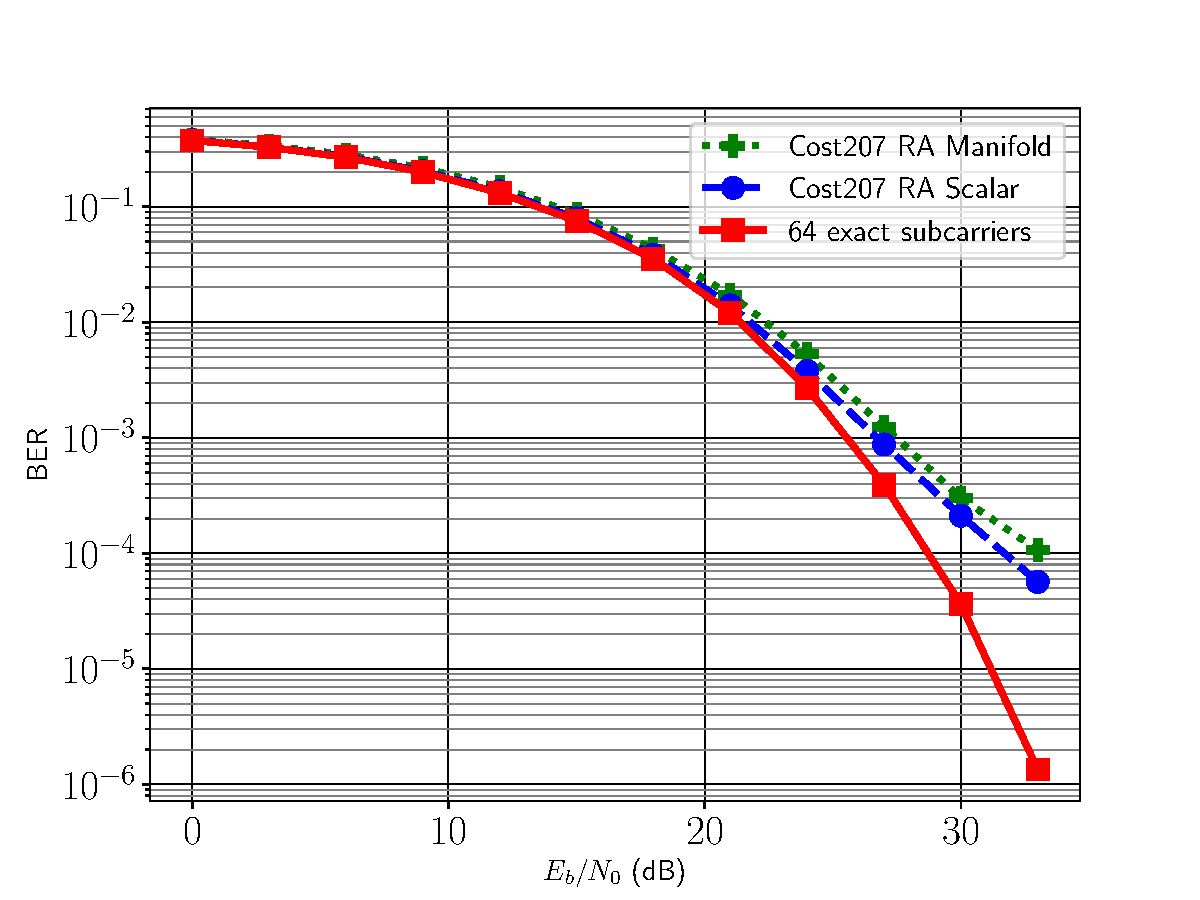
\includegraphics[width=0.5\textwidth]{images/ber64_001}
\caption{BER vs. SNR for QPSK transmission over the $4\times 2$ 64
  subcarrier MIMO-OFDM system, with the ITU Cost207-RA channel profile
  for $f_dT_s = 1.56\times 10^{-5}$, corresponding to a velocity of 172.8 km/h.}
\label{fig:ber_veh}
\end{figure}


% Since the Precoding matrices fundamentally lie on the Stiefel
% manifold, therefore, we are using the chordal distance parameter to
% measure the effectiveness of the quantization method used. Later we
% are comparing the BER rates with the completely fed back
% subcarriers. Or simulations and discussions part 2 criteria could be
% used. Done similar work as in \cite{4114278} but along with that we
% have joint interpolated in time and frequency at the transmitter using
% the fundamental scalar parameters obtained. To lower the number of
% bits we have used the method of interpolation and have achieved
% significant improvement over predictive quantization method in
% \cite{6891198} and also in \cite{Gupt1905:Predictive} which tried to
% use joint interpolation over the tangent space in the Stiefel
% Manifold. In fact, we use joint interpolation of the scalar parameters
% which are easy to use and give better quantization than any of the
% above methods.

% The advantage they had over the number of bits due to the 6 bit codebook in \cite{6891198,Gupt1905:Predictive} is also achieved by us by using smart interpolation techniques, i.e. by dropping the feedback bits in alternating time instances as it is still going to follow the scalar parameters without much difference.

% The problem of values hopping between $\pi$ and $-\pi$ is also tackled by wrapping the values around which we can show works nicely. The only drawback is that while initializing the parameter, they go out of their actual range and therefore using a uniform quantizer over the prescribed range does not work. But since most of the values lie between the given range we can use most of the initialization bits quantizing the parameters uniformly between the [-$\pi$ , $\pi$] and using smaller amount of bits between the range outside that which could go up to $-3\pi$ and $3\pi$, i.e. we are covering 300% more range outside the given area and that works mostly fine for the rest of the values.

% Using the idea of joint interpolation given in the other paper.

\section{Conclusion}
\label{section4}
We have presented a predictive quantization based precoder
reconstruction of a MIMO-OFDM system that employs scalar quantization
based feedback of precoder parameters. By quantizing and adapting the
Givens rotation and Householder transformation parameters of the
precoder, the receiver can send minimal feedback to the
transmitter and yet enable effective precoder adaptation. Exploiting
the temporal and frequency correlations jointly enhances precoder
accuracy significantly. Simulations reveal that the proposed approach
provides faster convergence and smaller errors in the precoder when
compared to approaches that involve direct quantization on manifold
tangent spaces. Future work would involve tuning the adaptation rate
of the scalar parameters and further reductions of quantization
redundancy to reduce the feedback rates.



% \section{Acknowledgment}

% % \label {section6}

% % \input{sections/6_section.tex}

% Parts of this work was supported by the Bharti Centre for Communication in

% IIT Bombay, and the Visvesvaraya

% PhD Scheme of Ministry of Electronics \& Information Technology,

% Government of India, being implemented by Digital India Corporation.





\renewcommand{\bibfont}{\footnotesize}

\bibliography{IEEEabrv,main}

\bibliographystyle{IEEEtran}

\end{document}
